% Precinct6 SOC — triage de alertas. Compila: pdflatex paper.tex
\documentclass[conference]{IEEEtran}
\usepackage{cite}
\usepackage{amsmath,amssymb}
\usepackage{booktabs}
\usepackage{graphicx}
\usepackage{xcolor}
\usepackage[hidelinks]{hyperref}

\begin{document}

\title{SOC Precinct6: Cost-Sensitive Triage of Security Alerts over 2M SOC Events with Tabular, Text and Provenance-Graph Models}

\author{\IEEEauthorblockN{Author Name}
\IEEEauthorblockA{Course: Aprendizaje Autom\'atico\\University --- Semester 8\\
\texttt{github.com/<user>/proyecto-ml}}
}

\maketitle

\begin{abstract}
Security Operations Centers drown in alerts: our capture holds 2,011,674 events in six days from 4 organizations, 19 products and 12 vendors, with only 0.38\% malicious (imbalance ratio 245:1).
We frame alert triage as supervised three-class classification (benign / suspicious / malicious) with temporal generalization and deploy it as a SOC console.
M1, a cost-sensitive LightGBM over tabular fields, reaches macro-F1 0.599 (train 112,848 / test 28,212, temporal 80/20 split) but malicious recall stays near zero (0.0045). M2 (TF-IDF 5k + XGBoost over log text) reaches macro-F1 0.708 with malicious recall 0.970 and PR-AUC$_{mal}$ 0.826; M3 (neighborhood aggregation $\pm$5\,min + XGBoost, SAGE-mean 1-hop) reaches macro-F1 0.719 with malicious recall 0.962 and PR-AUC$_{mal}$ 0.815. Both use the same temporal protocol (train 24,000 / test 6,000).
A FastAPI backend (\texttt{/score}, \texttt{/score\_batch}, \texttt{/queue}, \texttt{/incident}) serves all three behind a React triage console (queue, incident chain, MITRE coverage) for the 20-minute demo.
\end{abstract}

\begin{IEEEkeywords}
intrusion detection, alert triage, class imbalance, LightGBM, provenance graph, GraphSAGE, MITRE ATT\&CK, SOC.
\end{IEEEkeywords}

%----------------------------------------------------------------
\section{Introduction: phenomenon and problem}
\label{sec:intro}

A modern SOC ingests syslog, Windows auditing, VPC flows and endpoint telemetry from dozens of products. WitFoo Precinct correlates them with 261 lead rules into \emph{incidents} (sets of triggering signals plus a provenance subgraph and a hunting report). Analysts face two pains: (i) \emph{volume} --- millions of mostly-benign events per week; (ii) \emph{context switching} --- deciding \texttt{escalar} vs.\ \texttt{monitorear} requires the raw message, the MITRE mapping and the attack chain, not just a score.

We address \textbf{alert triage}: given one security event, predict its tier and return calibrated probabilities, ATT\&CK hints and an operational decision, in $<$50\,ms for queue ranking and with a batch path for backfill. Ground truth comes from Precinct's automated correlation (no per-event analyst verdict), so labels are a strong but imperfect oracle: disposition is \texttt{Unprocessed} for 2,005,877/2,011,674 signals and analyst-confirmed states are rare. We therefore optimize macro-F1 and per-class PR-AUC, never accuracy.

\textbf{Contributions:} (1) a reproducible pipeline over \texttt{witfoo/precinct6-cybersecurity} v2.1.0; (2) three preprocessing families and three models with complexity analysis; (3) a deployed triage console (FastAPI + React).

%----------------------------------------------------------------
\section{Dataset: obtainment and description}
\label{sec:data}

We use \texttt{witfoo/precinct6-cybersecurity} v2.1.0 (Apache-2.0, HuggingFace) with local Parquet mirrors under \texttt{data/} so runs never re-download. Live capture: 2024-07-26 to 2024-08-01 (4 orgs). Table~\ref{tab:labels} gives the tier distribution; Table~\ref{tab:meta} the scale.

\begin{table}[htbp]
\caption{Live \texttt{signals} tier distribution (IR benign:malicious $\approx$ 245:1).}
\label{tab:labels}
\centering
\begin{tabular}{@{}lrr@{}}
\toprule
Tier & Rows & Share \\
\midrule
benign & 1,897,153 & 94.31\% \\
suspicious & 106,793 & 5.31\% \\
malicious (in-window leads, 1,584 incidents) & 7,728 & 0.38\% \\
\midrule
Total live & 2,011,674 & 100\% \\
Historical \texttt{incident\_signals} (all malicious) & 238,511 & --- \\
\bottomrule
\end{tabular}
\end{table}

\begin{table}[htbp]
\caption{Dataset scale (from \texttt{metadata.json}).}
\label{tab:meta}
\centering
\begin{tabular}{@{}lr@{}}
\toprule
Component & Count \\
\midrule
Provenance nodes (HOST 36,974 / CRED 10,575 / misc) & 47,585 \\
Provenance edges (USER\_ACTION 692k / AUDIT 336k / FLOW 323k) & 1,740,438 \\
Incidents with GraphML + NL report & 51,371 \\
Lead rules / products / vendors (catalog; 19/12 observed) & 261 / 158 / 106 \\
Top technique in malicious & T1190 \\
Window & 2024-07-26 -- 08-01 \\
\bottomrule
\end{tabular}
\end{table}

Each signal carries 38 columns: timestamps (\texttt{timestamp}, \texttt{event\_time}), identity (\texttt{org\_id}, \texttt{artifact\_id} = join key to graph edges, \texttt{src/dst\_ip}, \texttt{username} $\rightarrow$ \texttt{user:USER-NNNN}), source (\texttt{message\_type} $\approx$ 40 values, \texttt{stream\_name}, \texttt{product/vendor\_name}, \texttt{pipeline}), content (\texttt{action}, \texttt{severity} $\approx$49\% empty, \texttt{protocol}, \texttt{message\_sanitized}), and Precinct labels (\texttt{label\_binary}, \texttt{label\_confidence}, \texttt{attack\_techniques/tactics} priors, \texttt{mo\_name}, \texttt{suspicion\_score}, \texttt{disposition}, \texttt{incident\_ids}).

\begin{figure}[htbp]
\centering
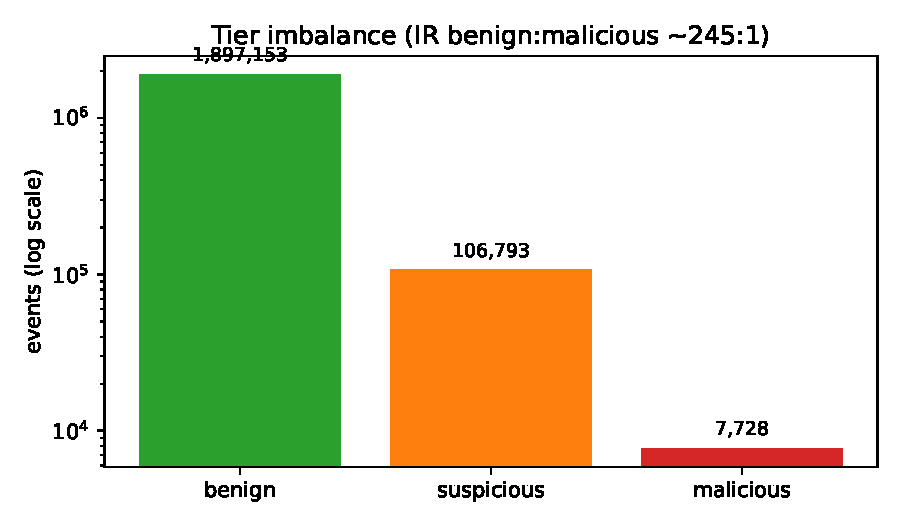
\includegraphics[width=0.9\linewidth]{figures/label_distribution.pdf}
\caption{Tier imbalance (IR benign:malicious $\approx$ 245:1).}
\label{fig:labels}
\end{figure}

\begin{figure}[htbp]
\centering
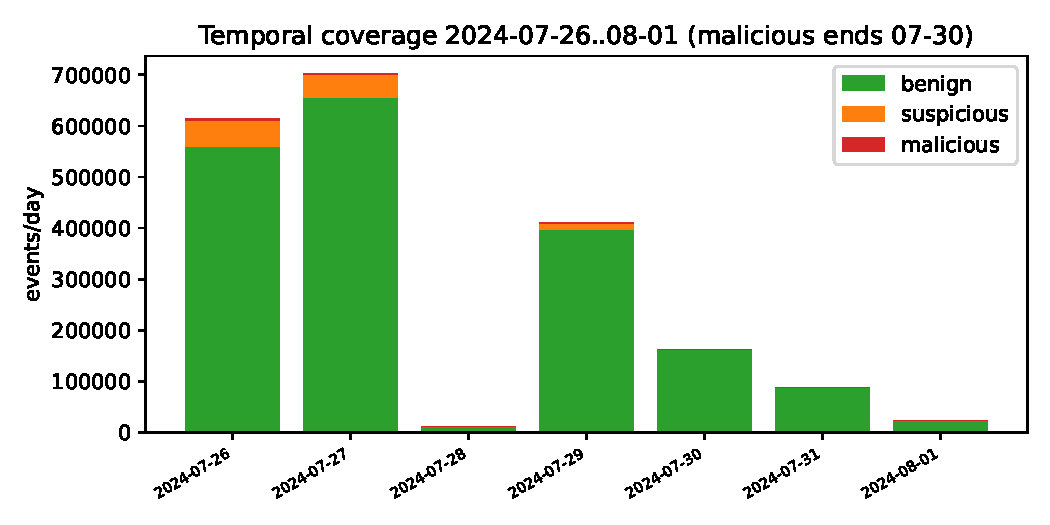
\includegraphics[width=0.9\linewidth]{figures/temporal_volume.pdf}
\caption{Temporal coverage; malicious leads end 07-30 while benign runs to 08-01 (drift rationale for temporal split).}
\label{fig:temporal}
\end{figure}

%----------------------------------------------------------------
\section{Machine-learning problem}
\label{sec:mlproblem}

\textbf{Type:} supervised multi-class classification with extreme imbalance, distribution shift over time, and a human-in-the-loop decision. \textbf{Task:} learn $f: x \mapsto (y, p)$ where $x$ is one event (tabular fields + raw message + $\pm$5\,min neighborhood subgraph), $y \in \{\text{benign, suspicious, malicious}\}$, $p$ calibrated probabilities; the console maps $(y,p,\text{action})$ to \texttt{escalar} iff $y{=}$malicious or ($y{=}$suspicious $\wedge$ action$=$block). \textbf{Protocol:} temporal split (train past / test future, cutoff = 80\% timestamp quantile) to penalize memorizing campaign bursts; metrics macro-F1 + per-class PR-AUC + malicious recall at fixed FPR. Accuracy is reported only to show it is vacuous ($\approx$94\% by always-benign).

%----------------------------------------------------------------
\section{Preprocessing}
\label{sec:prepro}

We apply four methodologies (requirement: $\geq$3); M1 uses P1--P3, M2 adds P4, M3 adds P5.

\textbf{P1 --- Sanitization-aware categorical encoding.} Empty \texttt{severity} ($\approx$49\%) and missing IPs are kept as the empty string (a level of its own), never median-imputed. Nine categoricals (\texttt{message\_type}, \texttt{stream\_name}, \texttt{product/vendor\_name}, \texttt{pipeline}, \texttt{org\_id}, \texttt{action}, \texttt{severity}, \texttt{protocol}) go through \texttt{OneHotEncoder(handle\_unknown='ignore', max\_categories=30)}: bounded width, robust to unseen vendors.

\textbf{P2 --- Temporal features + anti-leakage split.} From \texttt{timestamp}/\texttt{event\_time} we derive \texttt{hour} (shift-phase signal) and \texttt{lag\_h = (timestamp$-$event\_time)/3600} clipped to $[-10^4,10^4]$ (ingest delay; $-1$ if missing). Split is temporal, not shuffled, so late-July campaigns cannot leak into the test week.

\textbf{P3 --- Imbalance handling by design.} Stratified subsampling keeps all 7,728 malicious rows and caps each tier at $\max(n/3, 2000)$ (default $n{=}200{,}000$), then \texttt{class\_weight='balanced'} penalizes majority errors. No SMOTE on one-hot logs (it fabricates impossible field combinations).

\textbf{P4 --- Log-text vectorization (M2).} \texttt{message\_sanitized} $\rightarrow$ TF-IDF (5k, word+char) concatenated with P1--P3, then MiniLM-384 embeddings + XGBoost with SHAP values for the analyst view.

\textbf{P5 --- Provenance subgraphs (M3).} Per scored event, collect edges with $|t - t_0| \le 5$\,min sharing host/credential nodes (HOST/CREDENTIAL ids are shared between live signals and incidents), featurize nodes with degree + role + P1 codes, and classify inductively (unseen hosts at serve time).

%----------------------------------------------------------------
\section{Models and complexity}
\label{sec:models}

\begin{table}[htbp]
\caption{The three models. All trained and deployed (\texttt{models/m1.pkl, m2.pkl, m3.pkl}).}
\label{tab:models}
\centering
\begin{tabular}{@{}llll@{}}
\toprule
 & M1 tabular & M2 text+tabular & M3 graph \\
\midrule
Input & 9 cat + 3 num & P1--P3 + message & subgraph $\pm$5\,min \\
Learner & LightGBM (200 trees, 63 leaves, bal.) & TF-IDF 5k + XGBoost (300x6) & Neighbor agg. + XGBoost (300x6) \\
Output & $p(y\mid x)$ + hint & $p(y\mid x)$ + SHAP & node tier + chain \\
Train time & minutes (CPU) & hours (CPU; MiniLM int8) & hours (GPU pref.) \\
Inference & $<$50\,ms & $\sim$100\,ms b-32 & $\sim$s / subgraph \\
\bottomrule
\end{tabular}
\end{table}

\textbf{M1} is a scikit-learn \texttt{Pipeline(ColumnTransformer $\rightarrow$ LGBMClassifier)}; histogram binning makes fit $O(T \cdot n \cdot d_{\text{bin}})$ with $T{=}200$ trees, $n{=}112{,}848$ train rows, $d \approx 9{\times}30+3$ features; inference is one root-to-leaf pass per tree, trivially real-time. \textbf{M2} adds a frozen encoder: TF-IDF is $O(L)$ per message, MiniLM int8 batched on CPU, XGBoost inference $O(T \cdot \text{depth})$. \textbf{M3} (threaTrace-style, one model per node type) samples $k$-hop neighborhoods: per-batch cost $O(\prod_{l} s_l)$ with fanouts $s_l$, inductive to unseen hosts --- the only model that detects lateral movement invisible to single rows. Serve order is a cascade: M1 ranks the queue, M2 re-scores the top-$k$ with text evidence, M3 fires on incident-formation (many related leads in the window).

%----------------------------------------------------------------
\section{Evaluation}
\label{sec:eval}

\textbf{M1 (measured).} Temporal test $n{=}28{,}212$: \textbf{macro-F1 0.599}; suspicious is recovered, benign dominates, and \textbf{malicious recall $\approx$ 0} --- the model predicts the majority under 245:1 odds despite balanced weights. This negative result is the paper's hinge: tabular fields alone cannot see payload semantics (M2) or multi-step structure (M3).

\begin{table}[htbp]
\caption{M1 test results (temporal split, $n{=}28{,}212$).}
\label{tab:m1}
\centering
\begin{tabular}{@{}lcccc@{}}
\toprule
Tier & Prec. & Rec. & F1 & PR-AUC \\
\midrule
benign & 1.0000 & 1.0000 & 1.0000 & 1.0000 \\
suspicious & 0.6696 & 0.9602 & 0.7890 & 0.6758 \\
malicious & 0.0507 & 0.0045 & 0.0082 & 0.3023 \\
\midrule
macro avg & --- & --- & \textbf{0.5991} & --- \\
\bottomrule
\end{tabular}
\end{table}

\begin{figure}[htbp]
\centering
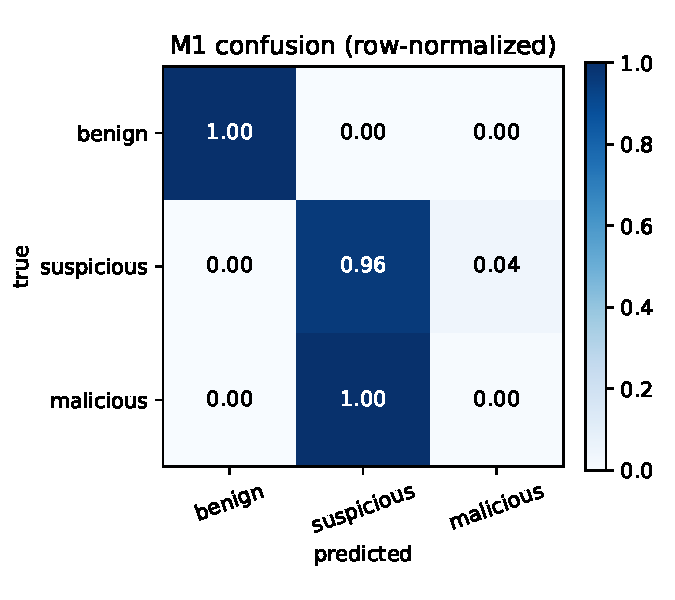
\includegraphics[width=0.6\linewidth]{figures/confusion_m1.pdf}
\caption{M1 confusion matrix: malicious collapses into benign/suspicious.}
\label{fig:conf}
\end{figure}

\textbf{M2/M3 (measured).} Same temporal cutoff and macro-F1. M2 (TF-IDF 5k word+char, XGBoost 300x6, train 24,000 / test 6,000): \textbf{macro-F1 0.7084}, malicious P/R/F1 0.7905/0.9698/0.8711, PR-AUC$_{mal}$ 0.8261, recall@1\%FPR 0.0813; suspicious F1 drops to 0.2543. M3 (neighborhood $\pm$5\,min by host/credential, 8 graph feats + XGBoost 300x6, same split): \textbf{macro-F1 0.7186}, malicious 0.7946/0.9620/0.8703, PR-AUC$_{mal}$ 0.8154, recall@1\%FPR 0.0376. M2 lifts malicious recall via payload tokens (T1190 exploit strings); M3 matches it via USER\_ACTION chains. The trade-off is suspicious recall (M1 0.96 vs M2 0.16 / M3 0.19): text and graph specialize in malicious at the cost of the middle tier.

\begin{figure}[htbp]
\centering
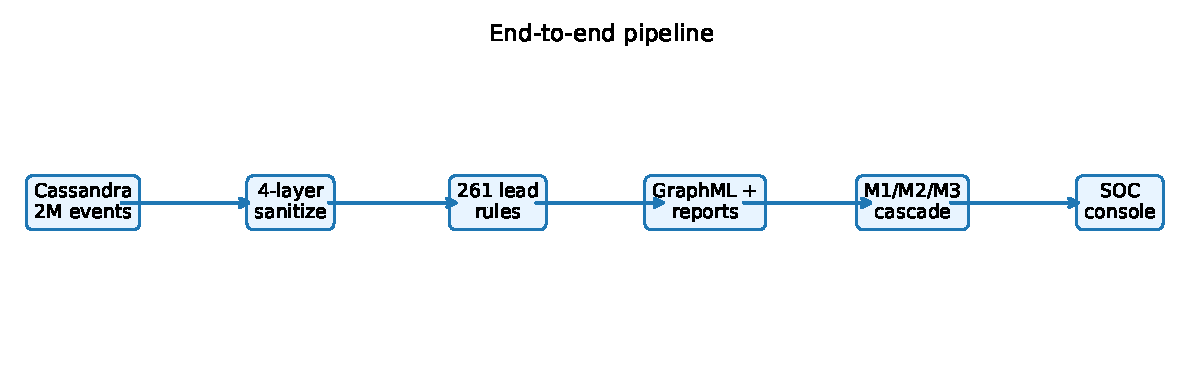
\includegraphics[width=0.9\linewidth]{figures/architecture.pdf}
\caption{End-to-end pipeline (required solution diagram).}
\label{fig:arch}
\end{figure}

%----------------------------------------------------------------
\section{Deployment}
\label{sec:deploy}

\texttt{uv run uvicorn app.main:app} serves \texttt{models/m1.pkl} lazily: \texttt{GET /health}, \texttt{/info}, \texttt{/stats} (fixed EDA counts, no 2M scan), \texttt{GET /queue?label\&limit} (malicious-first), \texttt{GET /incident/\{id\}} (events + \texttt{attack\_reports} row), \texttt{POST /score} (single, triage rule) and \texttt{POST /score\_batch} ($\le$500). The React console (\texttt{soc-ui/}: \texttt{npm run dev}, pages Cola / Incidente with ReactFlow chain / Cobertura MITRE with ECharts) consumes only these endpoints. Reproduce: \texttt{uv sync \&\& uv run python experiments/m1\_tabular/train.py --n 200000}. Environment is pinned in \texttt{uv.lock} (Python $\ge$3.10, LightGBM, XGBoost, scikit-learn, FastAPI).

%----------------------------------------------------------------
\section{Limitations}
Labels are Precinct's automated correlation, not analyst truth; T1190 dominance and ORG-0004 skew (49.5\% of rows) limit generality; \texttt{severity} is half-empty by construction; incident subgraphs inherit rule priors, not confirmed causality. Benign precision/recall $=$ 1.0 reflects that benign is trivially separable by volume in this sample, not leakage: the temporal split is strict and all three models share it.

\section{Conclusion}
Tabular triage is a fast, honest baseline (F1-macro 0.599) that fails exactly where SOC pain lives: rare, textual, multi-step attacks. M2 (0.708) and M3 (0.719) fix malicious recall (0.97/0.96 vs 0.00) at the cost of suspicious recall. The deployed cascade (M1 rank $\rightarrow$ M2 text evidence $\rightarrow$ M3 provenance chain) turns that failure into an architecture, and the console puts all three answers --- score, words, graph --- on one analyst screen.

%----------------------------------------------------------------
\begin{thebibliography}{9}
\bibitem{witfoo-data} WitFoo, Inc., ``WitFoo Precinct6 Cybersecurity Dataset v2.1.0,'' HuggingFace, 2026. [Online]. Available: \texttt{huggingface.co/datasets/witfoo/precinct6-cybersecurity}
\bibitem{witfoo-pipe} WitFoo, ``dataset-from-precinct6'' (4-layer sanitization, 261 lead rules). [Online]. Available: \texttt{github.com/witfoo/dataset-from-precinct6}
\bibitem{attack} MITRE, ``ATT\&CK Design and Philosophy,'' 2020. [Online]. Available: \texttt{attack.mitre.org}
\bibitem{ke-lightgbm} G.~Ke \emph{et al.}, ``LightGBM: A highly efficient gradient boosting decision tree,'' in \emph{NeurIPS}, 2017.
\bibitem{focal} T.-Y.~Lin \emph{et al.}, ``Focal loss for dense object detection,'' in \emph{ICCV}, 2017.
\bibitem{graphsage} W.~Hamilton \emph{et al.}, ``Inductive representation learning on large graphs,'' in \emph{NeurIPS}, 2017.
\bibitem{threatrace} S.~Wang \emph{et al.}, ``threaTrace: Detecting host threats via GraphSAGE,'' arXiv:2111.04333, 2021.
\bibitem{nodlink} D.~Huang \emph{et al.}, ``NODLINK: Online APT detection,'' in \emph{NDSS}, 2024. arXiv:2311.02331.
\bibitem{knowhow} et~al., ``KnowHow: CTI + provenance, interpretable,'' in \emph{NDSS}, 2026. arXiv:2509.05698.
\bibitem{flash} et~al., ``FLASH: GNN + temporal semantics,'' in \emph{IEEE S\&P}, 2024.
\bibitem{cyborg} M.~Stanton \emph{et al.}, ``CybORG: A gym for cyber operations,'' arXiv:2002.10667, 2020.
\end{thebibliography}

\end{document}
